%************************************************
\chapter{Chapter 2}\label{ch:chapter2} % $\mathbb{ZNR}$
%************************************************


%\begin{abstract}
%Although the use of computer vision to analyse images from smartphones is in its infancy, the opportunity to exploit these devices for various assistive applications is beginning to emerge. In this paper, we consider two potential applications of computer vision in the assistive context for blind and partially sighted users. These two applications are intended to help provide answers to the questions of ``Where am I?'' and ``What am I holding?''.
%
%\hspace{0.5cm}First, we suggest how to go about providing estimates of the indoor location of a user through queries submitted by a smartphone camera against a database of {\em visual paths} -- descriptions of the visual appearance of common journeys that might be taken. Our proposal is that such journeys could be harvested from, for example, sighted volunteers. Initial tests using bootstrap statistics do indeed suggest that there is sufficient information within such visual path data to provide indications of: a) along which of several routes a user might be navigating; b) where along a particular path they might be.
%
%\hspace{0.5cm} We will also discuss a pilot benchmarking database and test set for answering the second question of ``What am I holding?''.  We evaluated the role of video sequences, rather than individual images, in such a query context, and suggest how the extra information provided by temporal structure could significantly improve the reliability of search results, an important consideration for assistive applications.
%
%\keywords{Image-based localisation, path-planning, mobile assistive devices, object categorisation, mobile computer vision.}
%\end{abstract}

\section{Introduction}

Low vision brings many challenges to an individual, including reduced independence and social exclusion. The World Health Organisation estimates (2012) that more than 285 million people worldwide suffer from low vision or blindness. Due to changing demographics and greater incidence of disease -- e.g. diabetes -- blindness and failing sight are increasing in prevalence.  The cost to society includes direct health care expenditure, care-giver time and lost productivity.  Enabling people with visual impairment to increase participation will help address social exclusion and improve self-esteem and psychological well-being. There is the potential of near-commodity smartphones, backed by appropriate computer vision algorithms and supporting processes, to address this need.

\subsection{A Solution in Waiting?}
The growth in availability of camera-equipped smartphones, networks, methods of social networking and crowdsourcing of data offers new solutions to develop assistive systems that could be scaled in performance and capability\cite{Manduchi2012,Worsfold2010}. The services/capabilities that could be offered include:

\emph{Navigation}: GPS does not offer sufficient precision or reliability for indoor manoeuvring. A combination of visual cues, translated into speech or tactile information, is desirable.

\emph{Shopping}: Other challenges include shopping and product recognition, both in shops and at home. The technology for visual object recognition from mobile devices has arrived for sighted users: the challenges to deployment for visually-impaired users includes a) the existence of accessible label databases, that are free from commercial bias; b) changing retrieval algorithms and systems to place more emphasis on strong match confidence; c) techniques for conveying information readily to blind and partially-sighted users.

\emph{Personal Safety}: As a partially sighted user, one is faced with a number of hurdles when undertaking journeys away from a familiar environment, and lack of confidence about the ``unseen'' can be a significant contributing factor to reduced mobility.  Where does the pavement end?  Where is the entrance to the bus, and are there stairs?  Are there obstructions at head-height?   

In summary, the overarching need is to increase the possibility for independent living; in a hugely visually-oriented built environment, sighted users rely on visual cues, signage, and recognition of structures such as doorways.  Can these cues be reliably translated into semantically appropriate information using computer vision? Therefore we focus on the feasibility of answering two questions with existing technology from visual cues: ``Where am I?'' and ``What am I holding?''. 
%% 

%% WHERE AM I?

\section{Where Am I?}

Techniques for WiFi localisation are entering mainstream use through, at one level, estimates obtained from the physical locations of WiFi access points, simple measures of signal strength or approaches such as ``Walkie-Markie''~\cite{Shen}, which use multiple signatures to infer location.  These technologies hold great potential.  However, accurate localisation still relies strongly on reasonable accurate motion models, and the collection of other cues, such as accelerometry or gyroscopes \cite{Wang2012}.  

Indeed, no matter how good other sources of information are, few can replace the contextual information of visual inference.  During navigation, using natural vision, sighted individuals are able to {\em from one consistent information source}: a) recognise their location relative to previous journeys; b) locate entrances and exits; c) detect obstructions; d) recognise people; e) assess human intent;
f) identify objects or activities of personal interest.

Invoking computer vision to {\it simultaneously} solve all of these tasks is a current challenge.  Our purpose is to assess the feasibility and accuracy of existing computer vision techniques to meet some of these needs.  The primary question we address in this section relates to the first topic in the list above: can we use computer vision to recognise location against previous journeys.

\subsection{Related Approaches}
 
 Several methods of indoor localisation using smartphone-relevant technology have been described, including RSSI, dead-reckoning, and combinations for techniques that harvest environmental cues \cite{Wang2012}, \cite{Shen}. 
 
 Related approaches to this problem involve the use of techniques such as SLAM \cite{Durrant-Whyte2006} and PTAM \cite{Klein2009}. These methods are near state-of-the-art for monocular robot navigation, allowing geometry of a space to be mapped out dynamically at the same time that self-localisation is achieved.  Indeed, Pradeep and colleagues successfully applied this to a demonstration for indoor navigation in an assistive device \cite{Pradeep2010}.

\subsection{Visual Paths} 

 Methods such as SLAM and PTAM attempt to simultaneously map world geometry and localise a camera within that geometry.  Our question is slightly different: we seek to identify where we might be relative to previous journeys taken along the same route, either by ourselves or other people.  Thus, we introduce the idea of the {\it visual path}, a stream of descriptions captured from visual information as we traverse from location $A$ to location $B$, or from location $C$ to $D$. Such streams could be captured from the cameras of other users moving in the same physical space.

We can split the path localisation problem into two distinct tasks.  The first is to determine which of $P$ possible paths one is navigating along, and the second is to determine where along a particular visual path one is located.  In the context of computer vision, a key question concerns the {\it distinctiveness} of information along paths, either as indicators of a particular journey or as indicators of location along a known journey.  Note that we do not explicitly attempt to localise with respect to a map -- our suggestion is to localise with respect to a journey.  In the context of many users, this would appear to be a sensible way to harvest information about locations that might be frequently reconfigured in a manner that would reduce dependence on an explicit mapping processes.

Though SLAM and PTAM are strong candidates for assistive techniques, there is also the need to combine mapping with object detection.  Putting these systems in the category of mapping and localisation, we explore the possibility that rather than mapping out a space, a user might be more interested in merely following a path that has been traversed by others.  It is in this long-term, collaborative context that the visual path concept would sit: we wish to allow users to compare their journeys against those of others through these visual paths.

In tracing along different paths, we might ask how distinctive the visual content is along one path relative to the appearance along another. We used a standard keypoint and descriptor type approaches to describe visual paths captured by users as they walked along indoor environments.

We first studied the distribution of a similarity metric, $\gamma$, based on a modification of Lowe's ratio test for discriminating descriptors~\cite{Lowe2004}. The modification takes the form of an $L_{\infty}$-type normalisation on the distribution of squared Euclidean distances between distinctive descriptors that are close matches between database images along a set of $P$ possible paths $C_p,\,p=1,2,\ldots, P$.

\subsection{Visual Path Descriptions} First, consider a number $M_p^{(i)}$ of descriptor vectors, $\mathbf{v}_m^{(i)}, m=1,2,\ldots,M^{(i)}$ produced from an image, $\mathbf{I}^{(i)}_p$, with each vector being of  dimension $L \times 1$.  These descriptors are stacked into the rows of an $M^{(i)}\times L$ descriptor matrix, $\mathbf{V}^{(i)}_p$ associated with image $\mathbf{I}^{(i)}_p$.  A {\it set} of images, $\lbrace \mathbf{I}^{(i)}_p\rbrace_{i=1,2,\ldots\,N_p}$ is now collected for path $C_p$, and for each of these, a descriptor matrix is produced.  A visual path $C_p$ is then encoded by the set of matrices of descriptors, denoted $\mathcal{M}_p=\lbrace \mathbf{V}^{(i)}_p \rbrace_{i=1,2,\ldots,N_p}$ generated from the set of images taken along that path.
 
Query images, $\mathbf{J}^{(j)}$, $j=1,2,\ldots,N_q$ are now acquired, separately.  A particular query image is also mapped to matrix of descriptors $\mathbf{Q}^{(j)}$. We wish to know which of the $P$ paths the query image $\mathbf{J}^{(j)}$ has been taken on; this is answered by comparing the query descriptor matrix against the set of path descriptors for all paths, $\lbrace \mathcal{M}_p \rbrace_{p=1,2,\ldots, P}$.

\begin{figure}
\centering
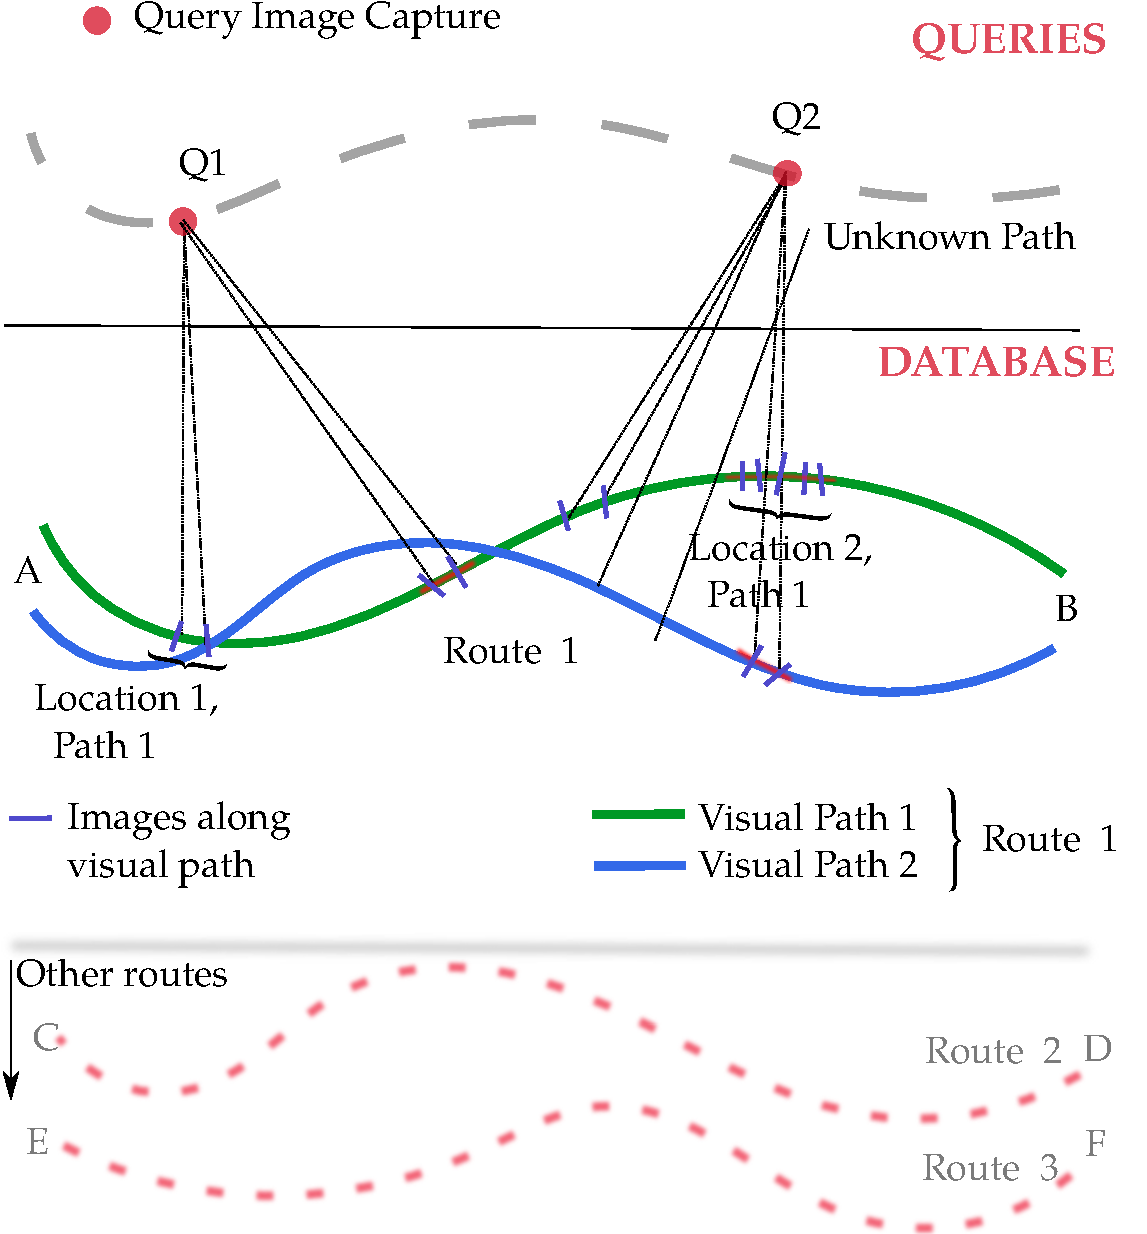
\includegraphics[width=\linewidth]{./gfx/Chapter02/pathexample.pdf}
\caption{Diagram illustrating the nature of visual paths and queries.  There are different paths recorded in the databases. The statistical tests reported in this paper compare the within-path queries and between-path queries, as well as within-path, between-location scores based on image comparisons.}
\label{fig:label}
\end{figure}


\subsection{Pairwise Descriptor Comparisons} \label{subsec:pairwise}

Let us first consider the comparison of individual query descriptors, $\mathbf{v}_n^{(j)}, n=1,2,\ldots,N^{(j)}$ arising from a single query image.  The Euclidean distance metric in $L$-dimensional space is widely used in assessing descriptor distances in computer vision.  Let $\mathbf{D}^{(i|n)}$ be the $M^{(i)}\times L$ matrix defined by

\begin{equation}
\centering
\mathbf{D}^{(i|n)}_p =  \mathds{1}_{M^{(i)}\times 1} \otimes \mathbf{v}_n^{(j)} - \mathbf{V}^{(i)}_p
\end{equation}

where $\mathds{1}$ is a vector of ones, and $\otimes$ denotes the Kronecker product.
Then the elements along the diagonal of

\begin{equation}
\centering
 \mathbf{D}^{(i|n)}_p[\mathbf{D}^{(i|n)}_p]^T
\end{equation}

are collated into a vector, $\mathbf{d}^{(i|n)}_p \in [0,\mathbb{R}^+]^{M^{(i)}}$ of squared Euclidean distances between the $n^{th}$ descriptor from a query image and each of the $M^{(i)}$ descriptors derived from the $i^{th}$ image along the path $C_p$. 

\subsection{Query Descriptor Rejection} \label{subsec:querydescrejection}
Many descriptors in the query image will not be sufficiently distinct to be useful in matching.  The distribution of distances contained in vector $\mathbf{d}^{(i|n)}_p$ is used in a first stage filtering for distinctiveness by order-statistic filtering.  A query descriptor $\mathbf{v}_n^{(j)}$ is considered suitable for use in assessing similarity between a pair of images only if $d^{(i|n)}_{[1]} < \alpha \cdot d^{(i|n)}_{[2]}$ where $d^{(i|n)}_{[1]}, d^{(i|n)}_{[2]},\ldots $ denotes the sorted elements of the vector $\mathbf{d}^{(i|n)}_p$ in increasing order (the path subscript $p$ is temporarily suppressed to include the order-statistic of elements).  $0<\alpha<1$ is set to around 0.7, and any {\it query} descriptors that do not satisfy this condition are discarded. All image query vectors are subjected to the same test.  Those that pass the test allow an ``average'' distance based on best matching descriptors to be used to determine how close a single query image is to a single database image.  That is, for a single image query  we  calculate

\begin{equation}
\centering
\mu^{(i,j)}_p=\frac{1}{|\mathcal{D}|}\sum_{n\in \mathcal{D}} d^{(i|n)}_{[1]}
\end{equation}

where $\mathcal{D}$ is the set of query descriptors that pass the distinctiveness test, as described here. Again, note that path subscript $p$ has been omitted from the right-hand side of this expression to represent the sorted distances.

\subsection{The $\gamma$ Score} We calculated  $\mu_p^{(i,j)}$ across all query images $\mathbf{J}^{(j)}$, $j=1,2,\ldots,N_q$ and all path images $\lbrace\lbrace I^{(i)}_p\rbrace_{i=1,2,\ldots,N_p}\rbrace_{p=1,2,\ldots P}$.   A $\gamma$ score is then defined to produce a score, $\gamma^{(i,j)}$, as a measure of similarity between image pairs $(i,j)$ relative to path $p$ such that $0 < \gamma \le 1$. 


\begin{equation}
\centering
\gamma^{(i,j)} = \frac{||\mu^{(i,j)}_p||_{\infty}-\mu^{(i,j)}_p}{||\mu^{(i,j)}_p||_{\infty}}
\end{equation}

The $\gamma$ measure is applied between pairs of query and database images, and one may identify two types of categories that these query comparisons fall into.  In the first case, the images come from the same path (although query and visual path database are, of course, distinct).  In the other case, queries come from different paths.  The results are shown in Fig.~\ref{fig:gammaDistribution}.   

\begin{figure}[ht]
\centering
{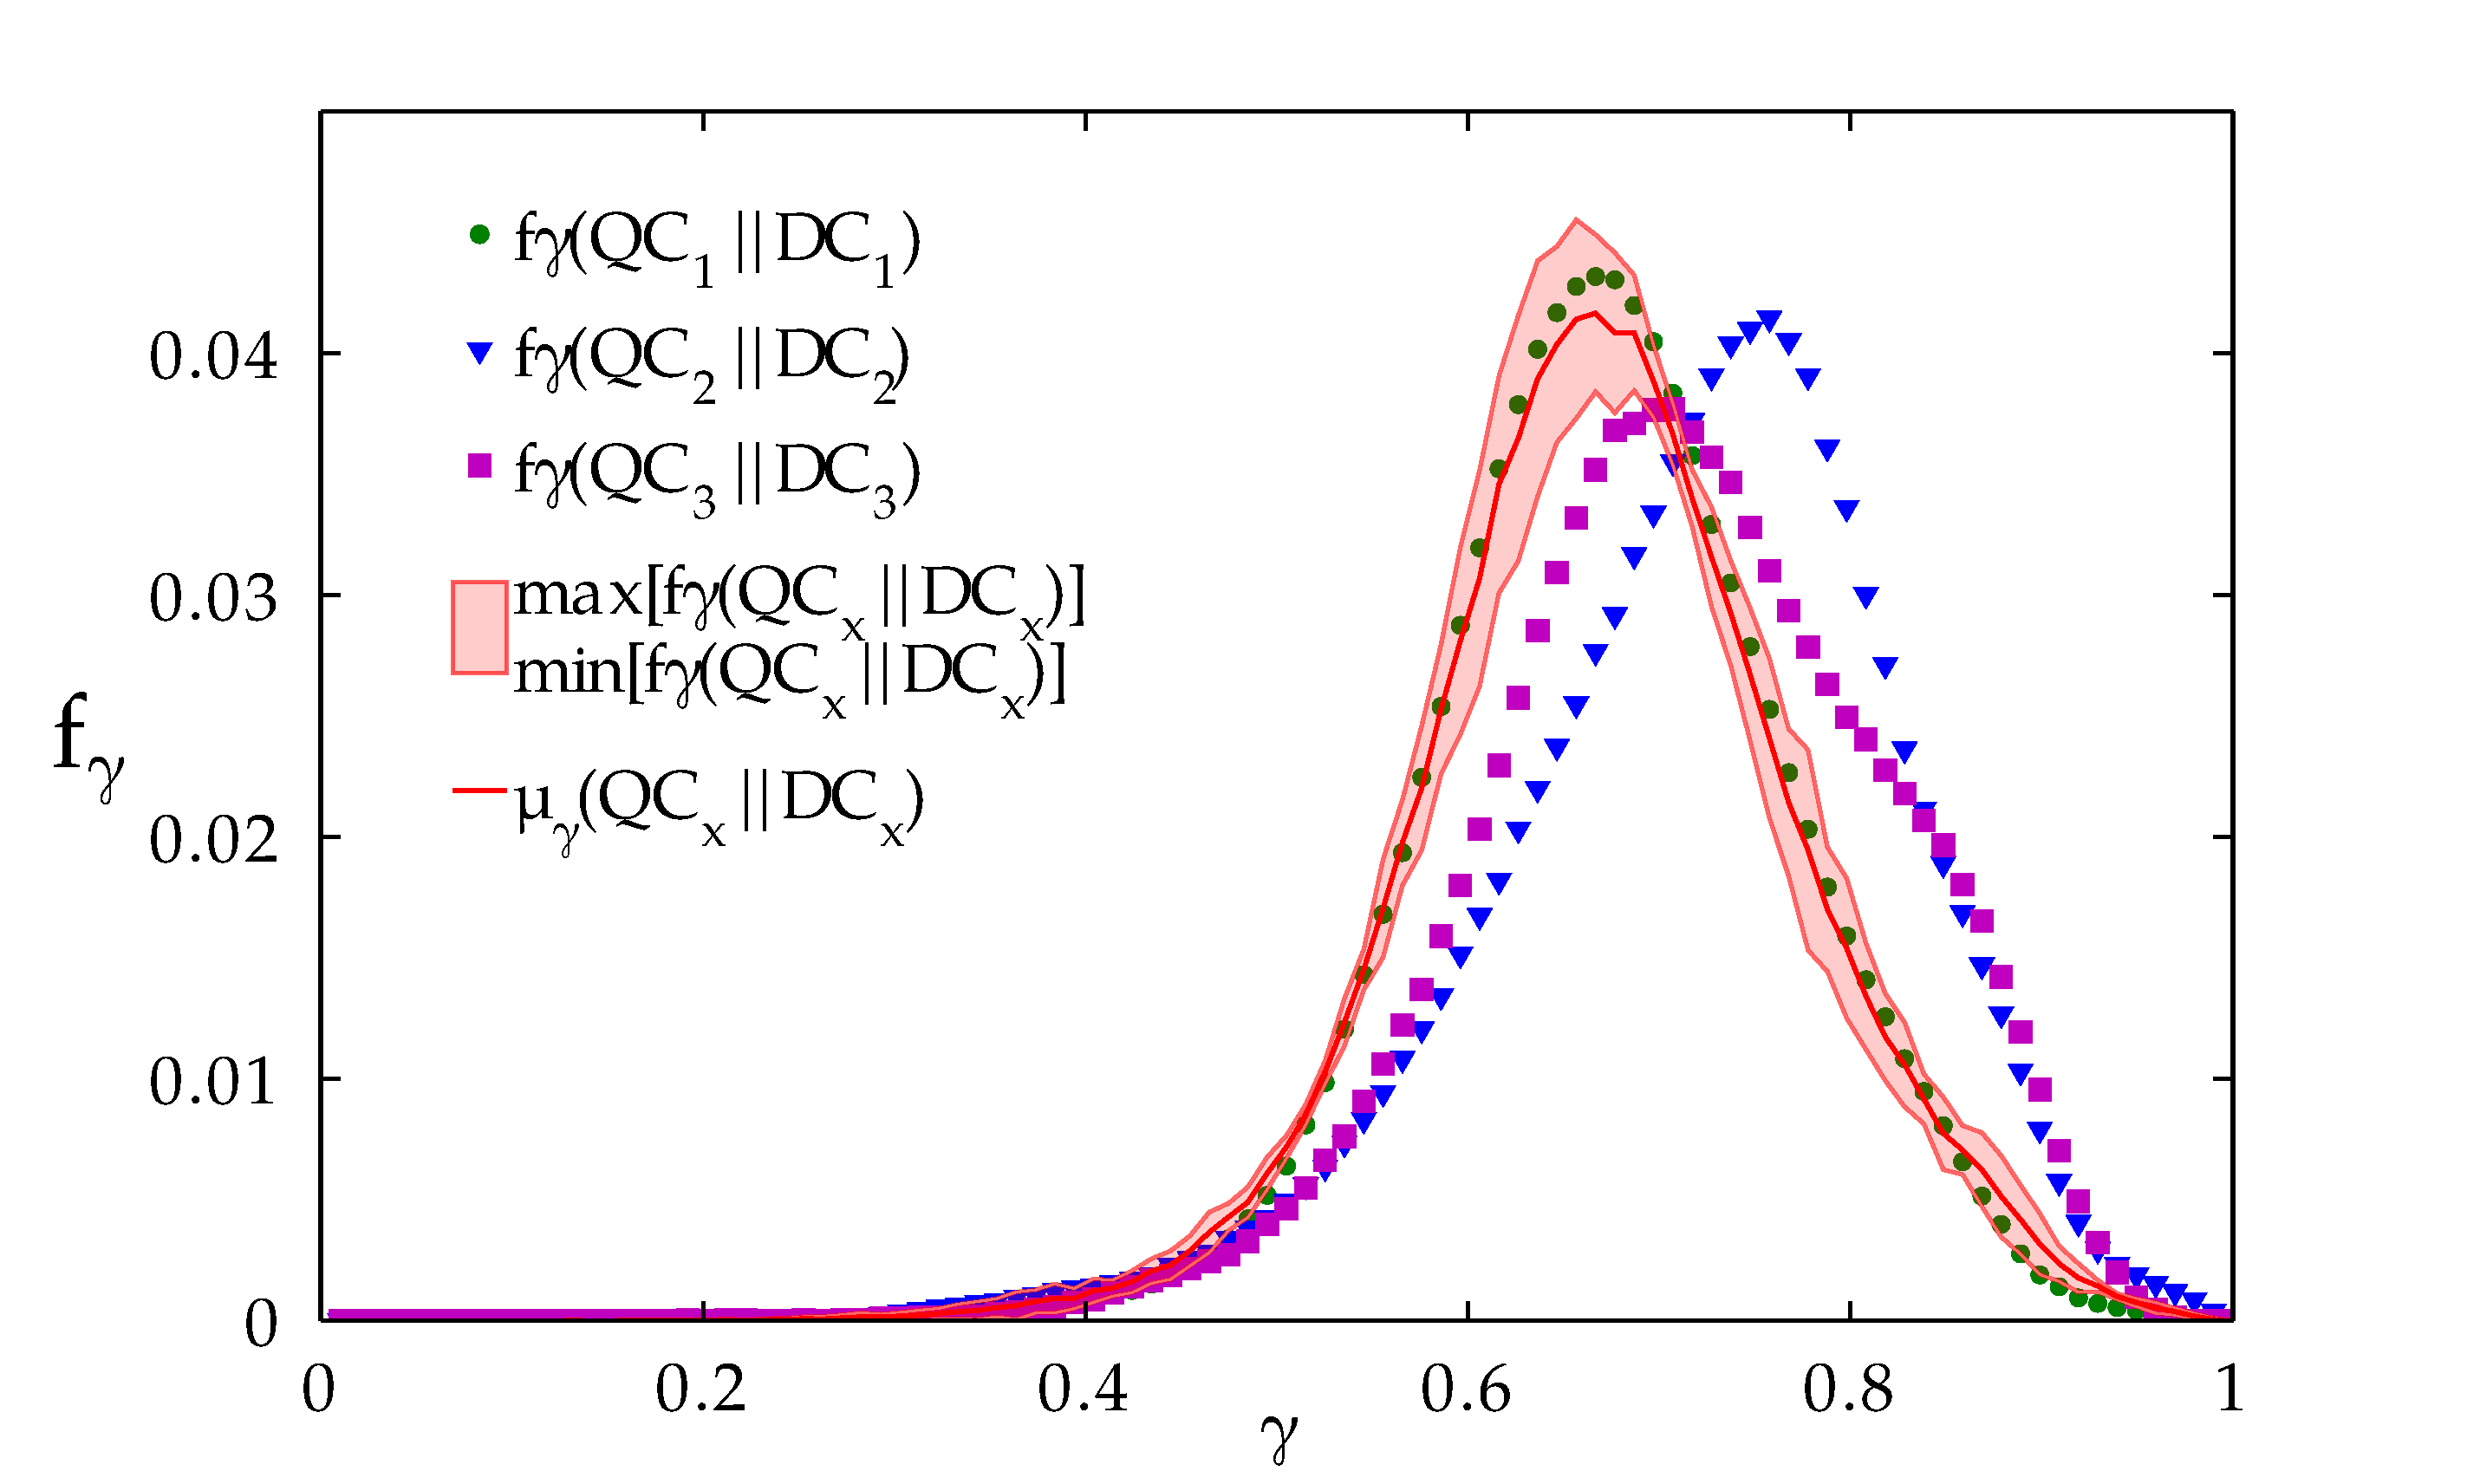
\includegraphics[width=\linewidth]{./gfx/Chapter02/path_pdf_analysisWithShadedBetweensALLDB.pdf}}
\caption{Tests of visual distinctiveness along paths: Distributions for the $\gamma$ metric. Path level queries, capturing the behaviour of the $\gamma$ metric for inter- and intra-path distributions.}
\label{fig:gammaDistribution}
\end{figure}
 



A second type of score, $\rho$, was created with a slightly different normalisation criterion based on observing the maximum within-path distance distributions, i.e. for a given path index, $p$.  The behaviour of this score was studied using query images as taken with ground-truth locations, measured with a surveyor's wheel; again, probability density estimates of scores are estimated from hundreds of thousands of descriptor comparisons.


\begin{figure}[ht]
\centering
{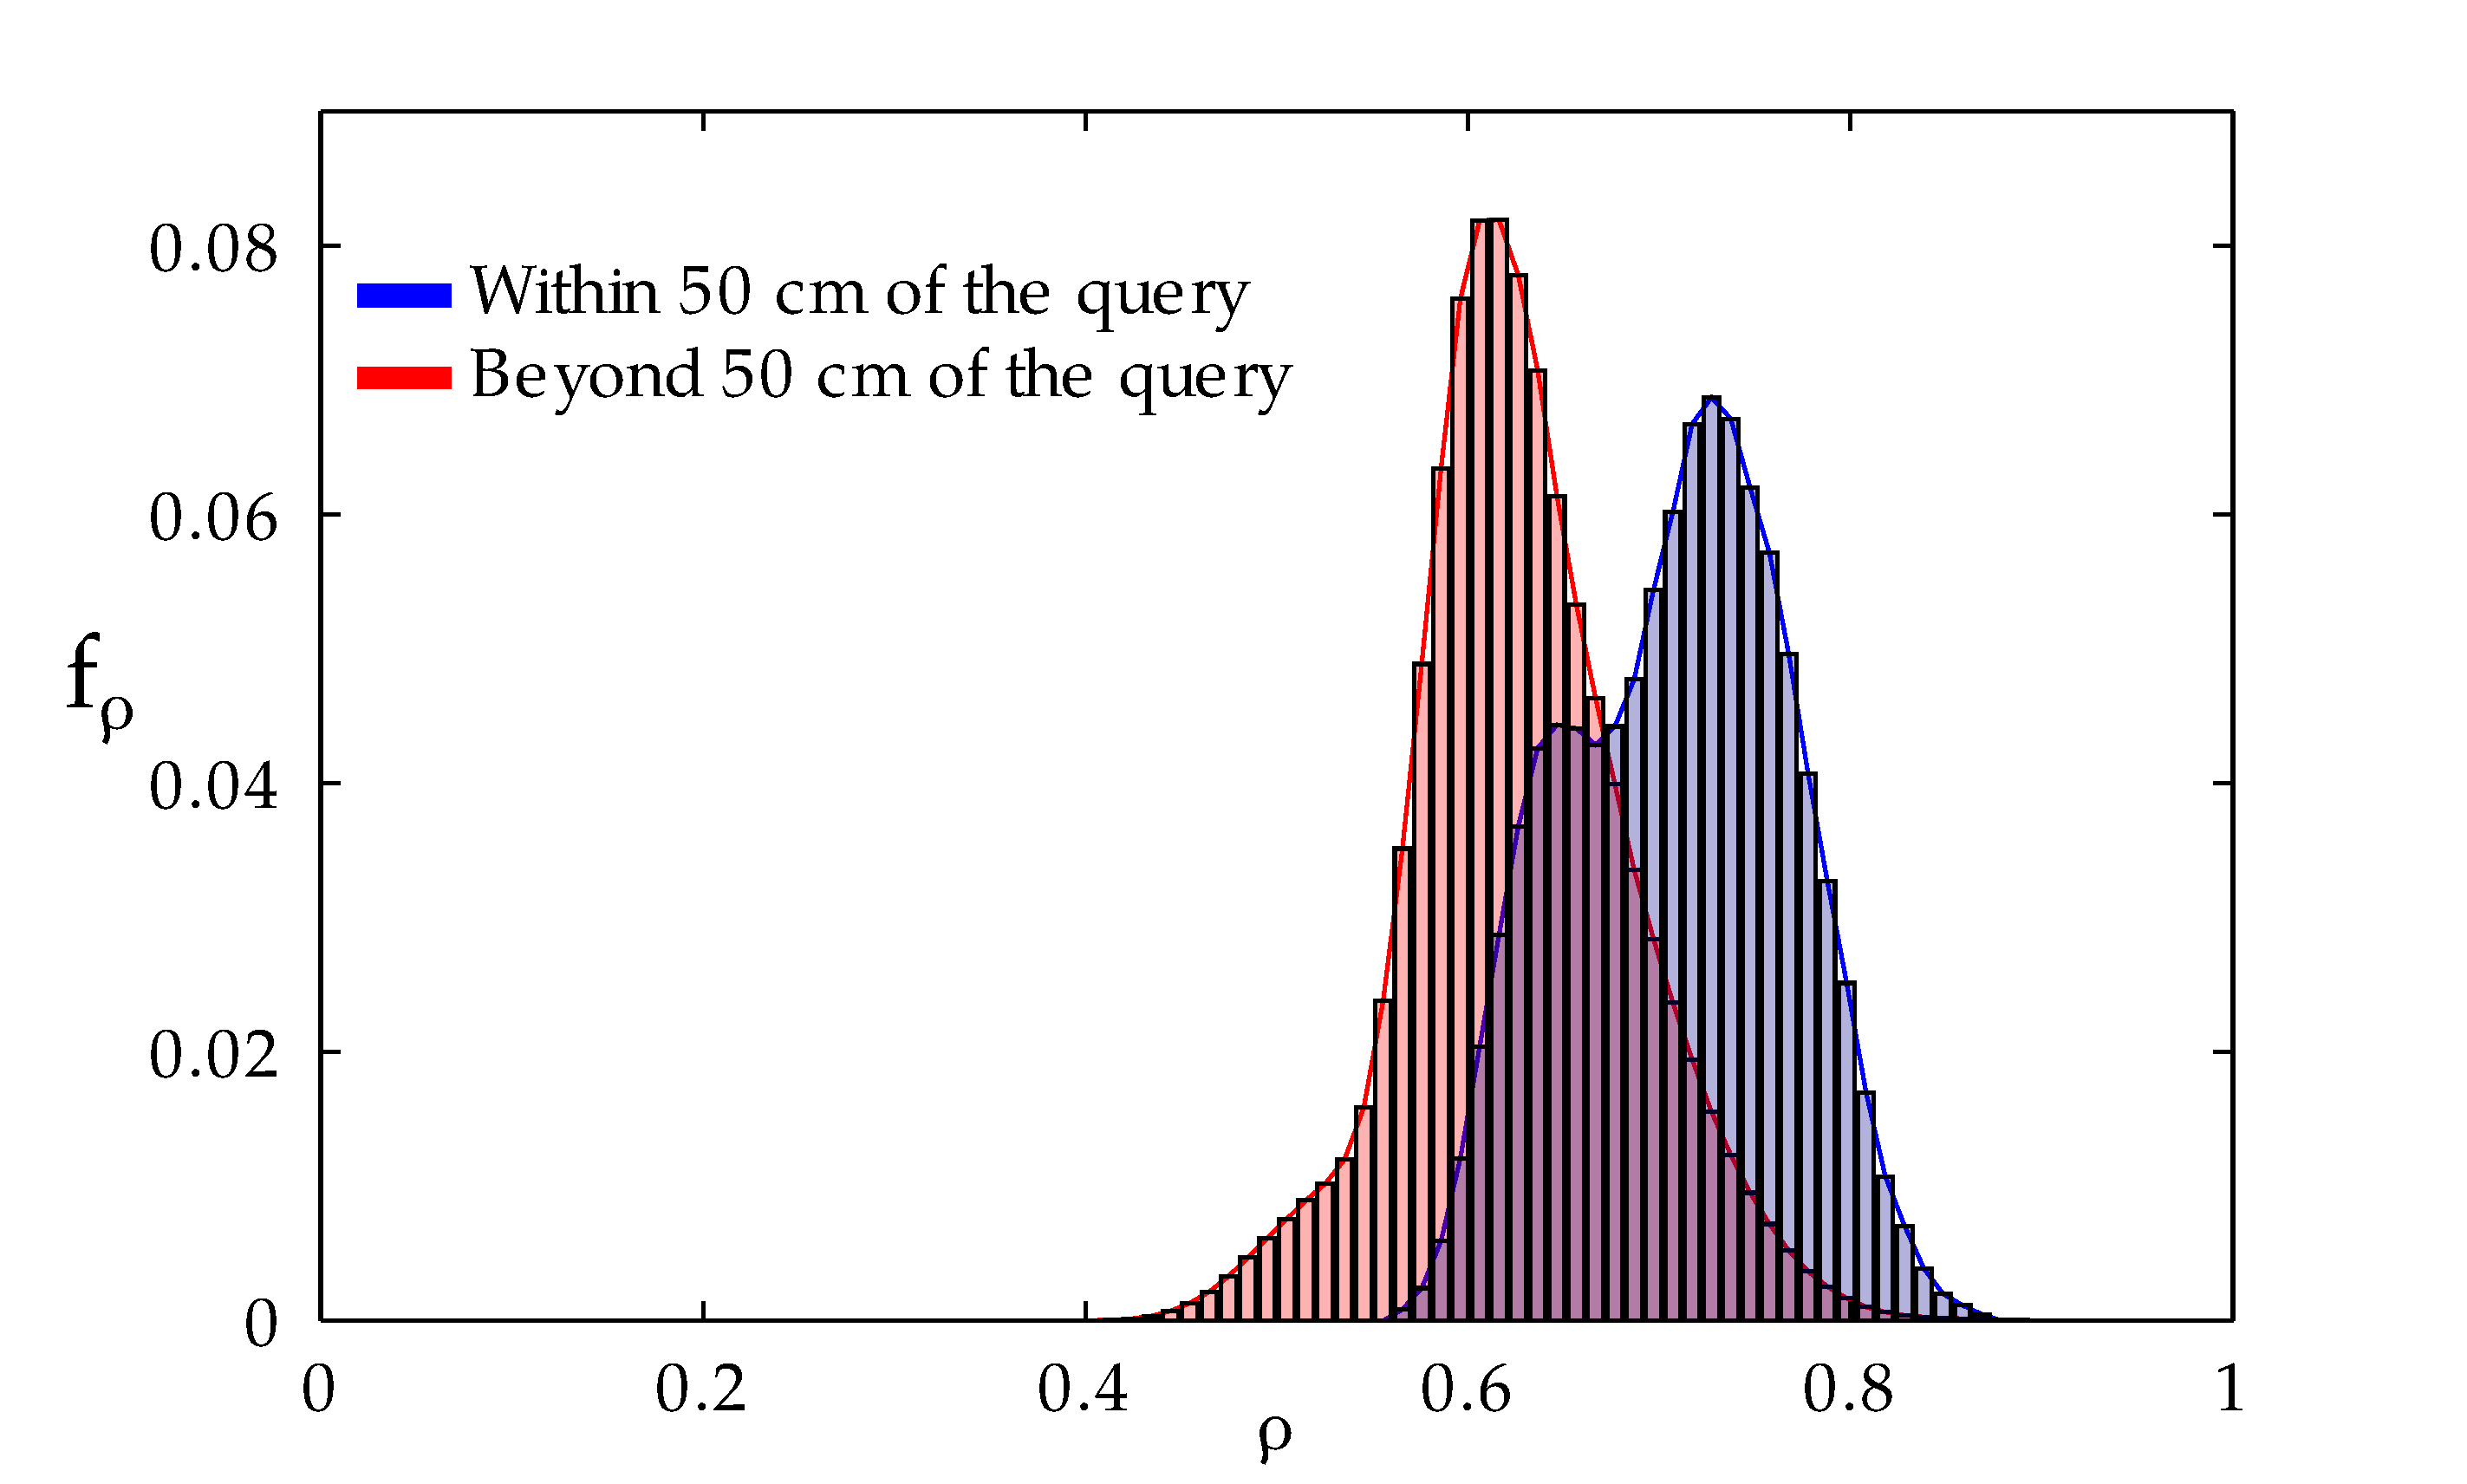
\includegraphics[width=\linewidth]{./gfx/Chapter02/C5distributions_no_smoothingWithSmoothedHistograms-latex.pdf}}
\caption{Tests of visual distinctiveness along paths: Distributions for the $\rho$ metric. Locations within a path, illustrating the distribution trends of the $\rho$-metric, all within a single 80m path, but at different distances either within or outside 50cm from known query submissions.}        
\label{fig:rhoDistribution}
\end{figure}

%%

%% WHAT AM I HOLDING?

\section{What Am I Holding?}

An increasing use for smartphones involves using {\it visual search} in which a photograph taken with the phone is used as a query into a catalogue of database items.  Common items include paperbacks (books), compact-disc packaging and, increasingly, art.  A closely related approach is the use of barcodes on items to look up both price information and more detailed product information.  

For the visually impaired, barcodes may be difficult to locate, and one would wish to allow recognition on objects and products from different points of view. The quality of a query image might also be below that of a sighted user.  For this reason, it is appropriate to assess the ability of visual search algorithms, designed for large-scale categorisation, to perform when the image queries are of low quality, as might occur in poor or variable lighting conditions.

The SHORT database~\cite{Rivera-Rubio2013a} provides such a dataset; and though it lacks the category-level complexity of real-world product databases, it is compliant with other datasets used in computer vision, such as the Pascal VOC database~\cite{Everingham2009}.  SHORT includes data acquired from 20 different smartphone cameras, with varying degrees of resolution and image quality.  An example of typical queries is shown in Fig.~\ref{fig:ShortQueries} below.

\begin{figure}
\centering
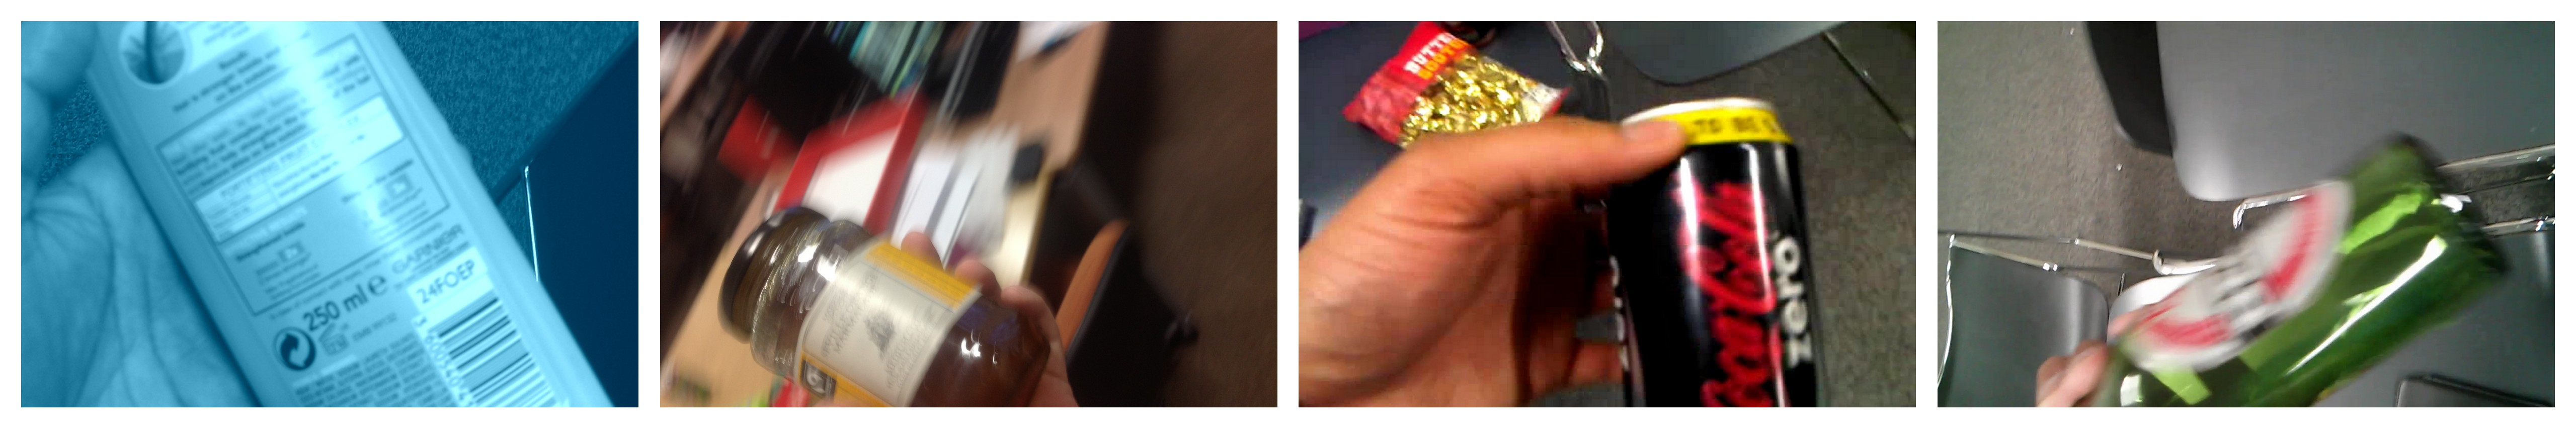
\includegraphics[width=\textwidth]{./gfx/Chapter02/TestDatasetCollage4imgs.jpg}
\caption{The SHORT database contains thousands of query images that form a representative set of examples of smartphone queries containing everyday household or packaged food products.}
\label{fig:ShortQueries}
\end{figure}
The dataset contains a mixture of stills and video clips, including more than 55,000 video frames and more than 1,900 still images.  Image sizes range from under 100,000 pixels to over 6 megapixels.


\subsection{Evaluation of Sequential Video Frames} \label{subsec:evaluationframes}

In this section we analyse how we can use sequential frames from a video of an object in order to improve classification accuracy. First, multiple sequential images from a video were queried, and each image was matched to one of the thirty categories of the SHORT-30 database using the descriptor matching as described in Sections~\ref{subsec:pairwise} and \ref{subsec:querydescrejection}. A histogram of the matches was computed for several videos of the same object, as shown in Fig.~\ref{fig:prd003a}. Even though the total number of incorrect matches increases as we query more video frames, they are distributed across a range of object categories in the database. 

\begin{figure}[t]
\centering
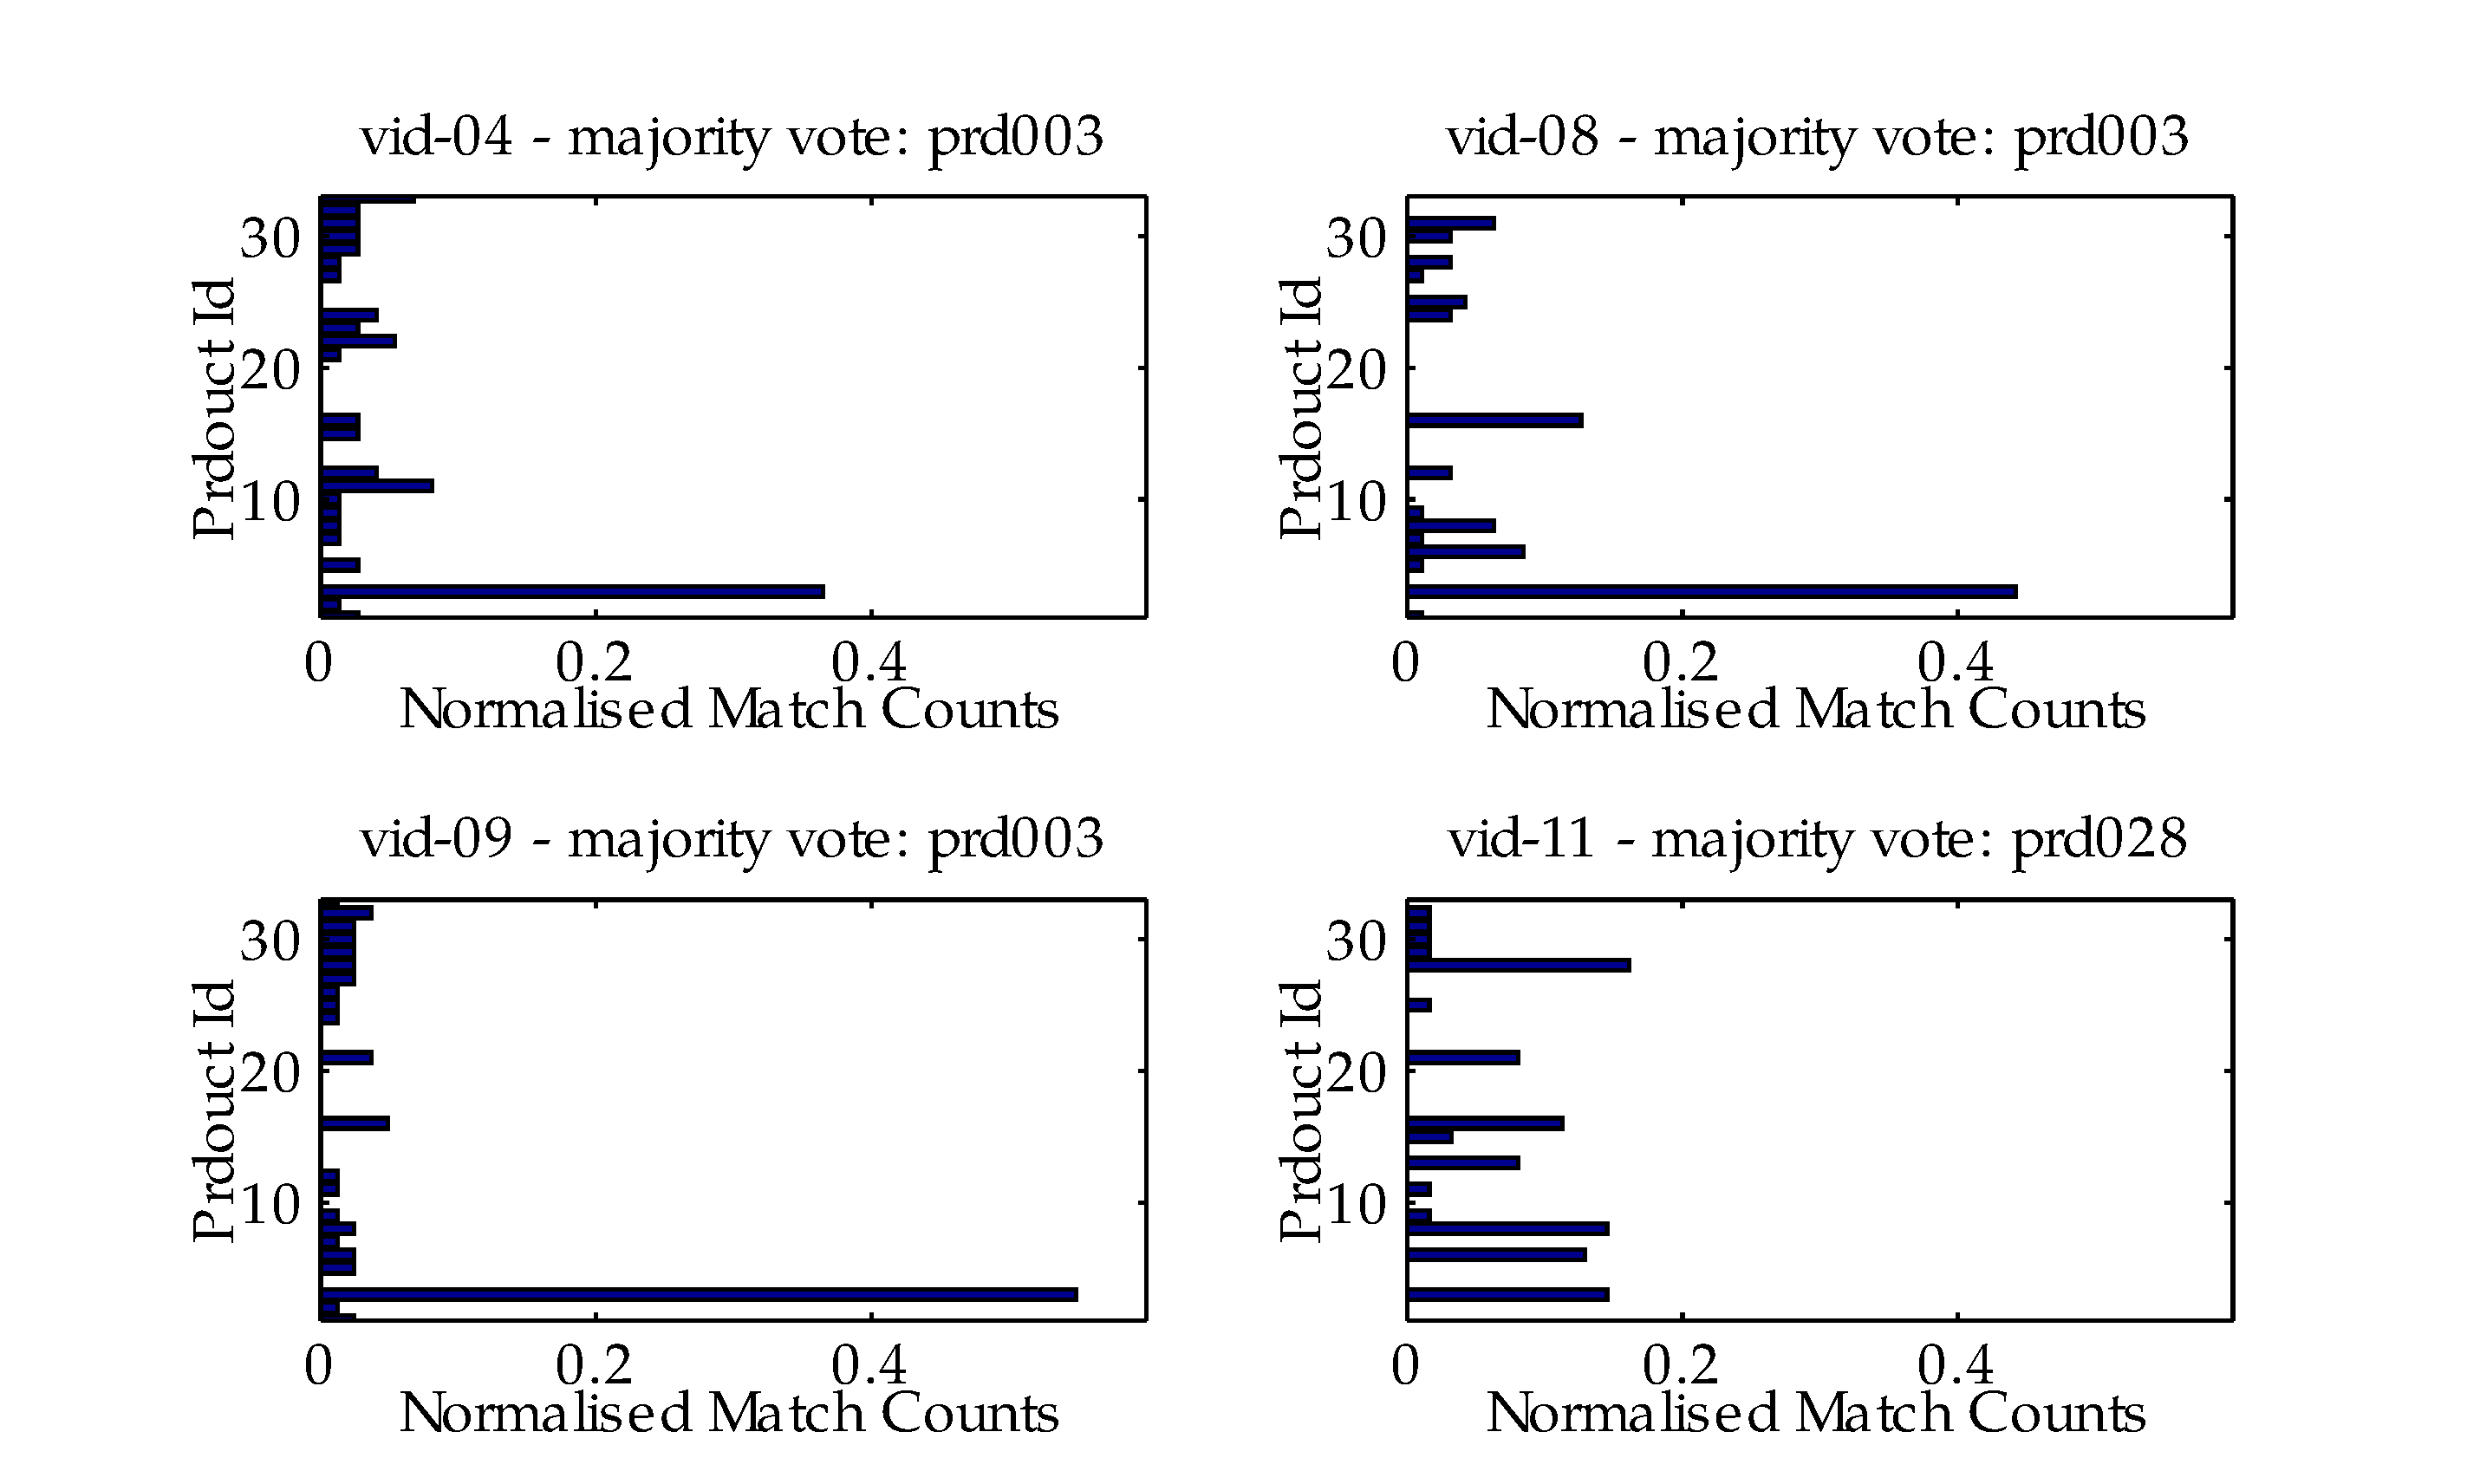
\includegraphics[width=\linewidth]{./gfx/Chapter02/prd003_distribution_bar-latex.pdf}
\caption{Evaluation of sequential video frames: Distribution of matches across different categories of SHORT-30 dataset for four videos of the same query object.}
\label{fig:prd003a}
\end{figure}


As shown, the correct object often has a higher number of hits than the incorrect ones. Therefore we propose to use the ``individual voting'' as a metric to classify an object based on querying sequential images from a video of a hand-held object. Further analysis was undertaken in order to determine the number of video frames that are required for the total number of correct matches to exceed the number of individual total incorrect matches. Preliminary results, Figure \ref{fig:prd003b}, shows that the number of total incorrect matches to individual objects rises slowly while the number of total matches to the correct object increases rapidly. The above analyses were undertaken for several videos and object categories under the SHORT-30 dataset. Classification accuracy using different numbers of query frames and the above metric is presented in Section~\ref{sec:expResults2}.


\begin{figure}[t]
\centering
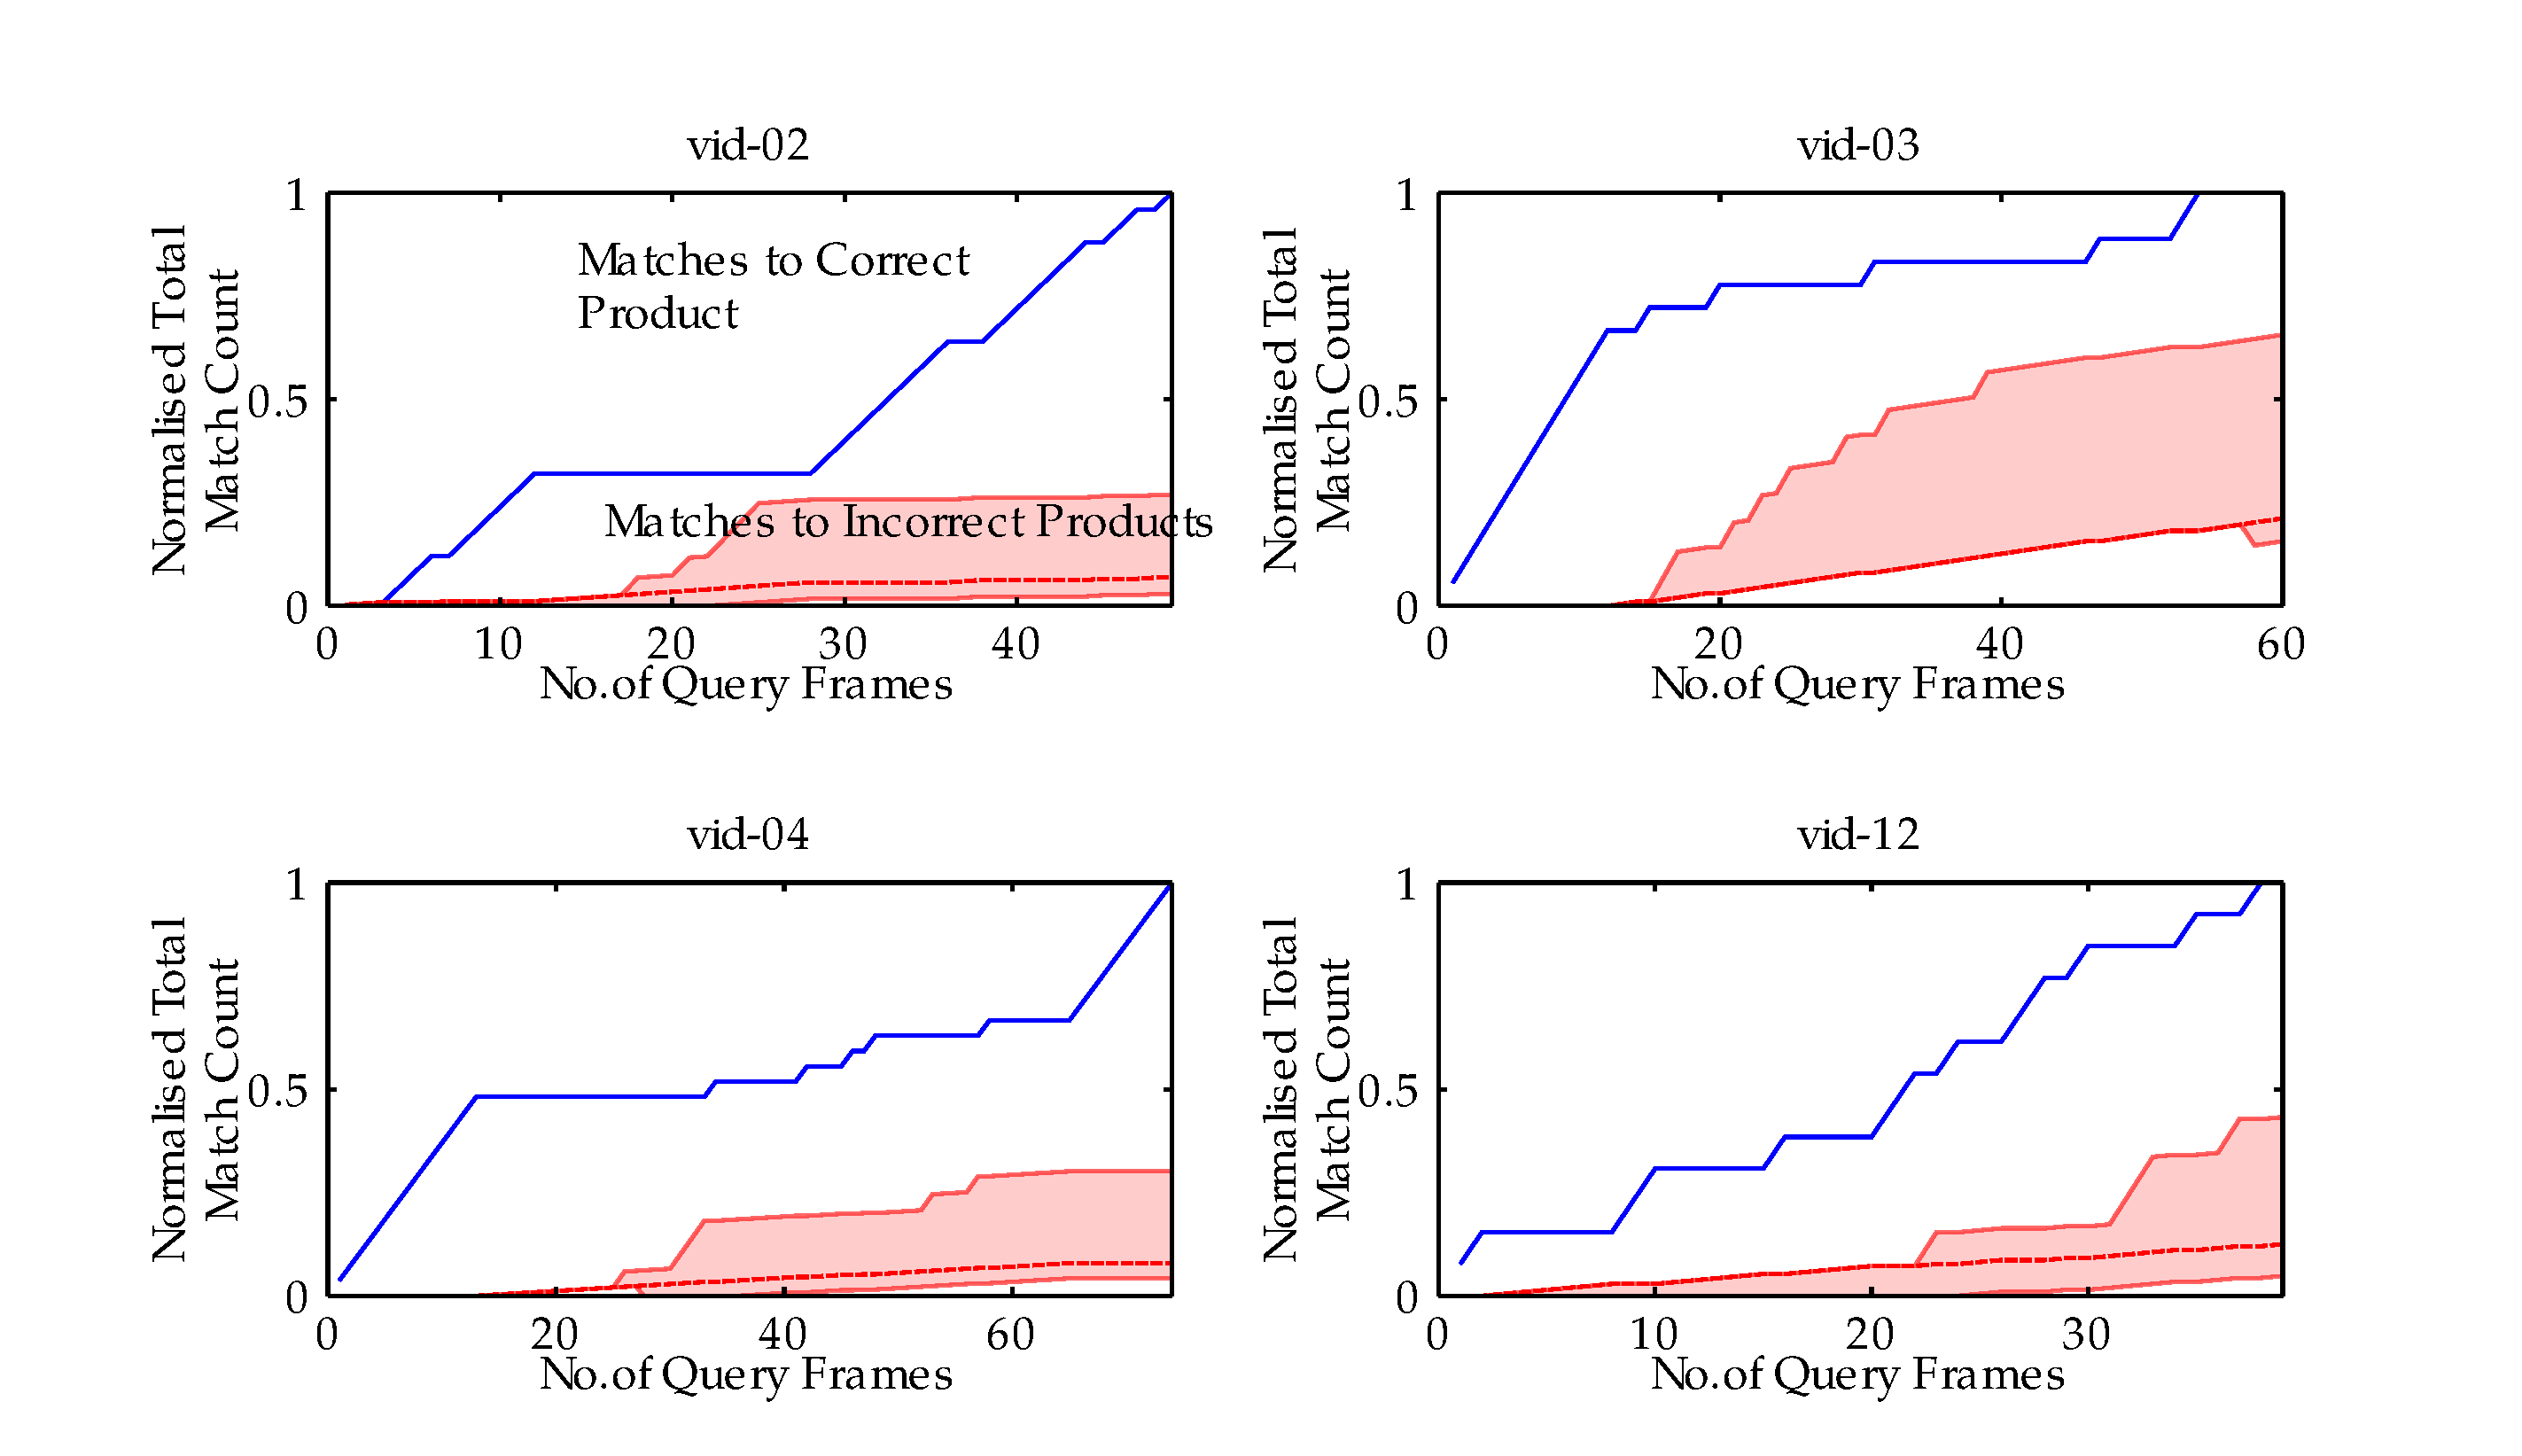
\includegraphics[width=\linewidth]{./gfx/Chapter02/prd0030shadedPlots-4-latex.pdf}
\caption{Evaluation of sequential video frames: Fraction of correctly matched queries to incorrect matches for videoframe sequences. Note that there is a distribution of incorrect matches across multiple categories as the number of sequential query frames increases.}        
\label{fig:prd003b}
\end{figure}


\section{Experimental Results} \label{sec:expResults}

\subsection{Navigation}

We acquired a number of visual paths with a mobile phone (Nexus 4).  These simply take the form of video acquisitions, captured with the phone pointing in the direction of motion, and recording at 30fps at 1920 $\times$ 1080 resolution. The images were then downsampled to a resolution of 192 $\times$ 108 pixels. The number of images captured along the paths raises the complexity of the image matching problem task: there are typically 2000 images per path.

For the analysis of the distribution of the metrics $\gamma$ and $\rho$, as shown in Fig.~\ref{fig:gammaDistribution} and \ref{fig:rhoDistribution}, we have used VLFEAT's~\cite{Vedaldi2008} implementation of SIFT~\cite{Lowe2004} descriptors.

\begin{figure}
\begin{center}
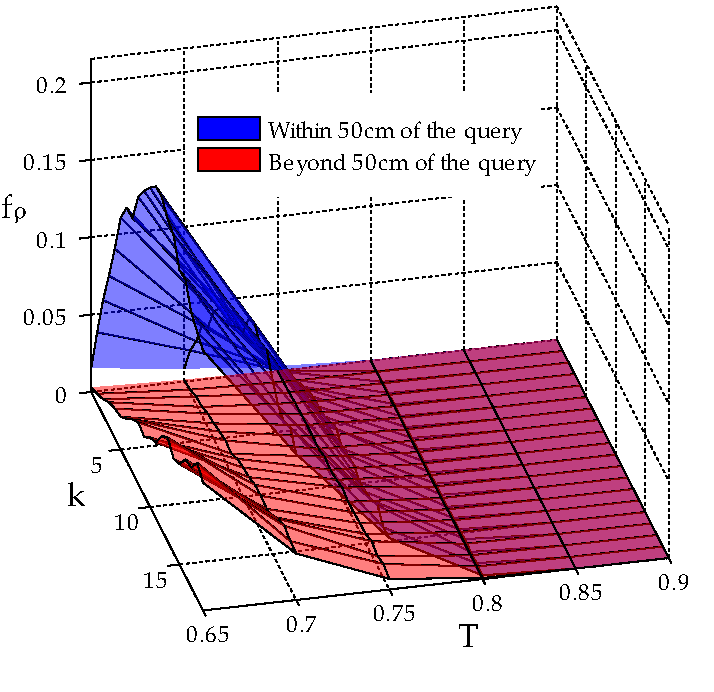
\includegraphics[width=.8\linewidth]{./gfx/Chapter02/C1twoTestWithBootstrapping2.pdf}
\caption{Fraction of values of $\rho$ exceeding a threshold $T$ in $k$ consecutive database frames.}
\label{fig:rocTwoParametersC5}
\end{center}
\end{figure}

The use of bootstrap statistics was appropriate for this study because, for example, in the navigational context, it allows sampling distributions of distances across the whole image database of around 400,000 possible pairings of visual path images.

In the case of the $\rho$ metric, these bootstrapped measurements have revealed the existence of visual distinctiveness between positions that are ``close'' or ``far'' along a path from a given query. In Fig.~\ref{fig:rhoDistribution} we have double-filtered the distribution of the $\rho$ values with a one-point moving average. This clearly shows that values of $\rho$ closer to one are useful for discriminating positions belonging to a specific visual path. These results have motivated the search for a threshold on the values of $\rho$ and the use of consecutive database frames to maximise discriminability, as illustrated in Fig.~\ref{fig:rocTwoParametersC5}.

\subsection{Classification Accuracy Based on Sequential Video Frames} \label{sec:expResults2}

Classification accuracy using the individual voting metric (Section~\ref{subsec:evaluationframes}) was computed for six categories of SHORT-30 dataset (Table~\ref{table:testData}). A video $\mathbf{Q}$, comprising of query frames $Q_i, i = 1,2,...,N$, is classified as the $k$-th category, $C_k$, to which the majority of query frames, $Q_i$, were matched to. The accuracy was calculated for classifying twelve videos of each object based on different limits for the number of queries allowed, $N$.

Table~\ref{table:testData} shows that the classification accuracy increases as we increase the limit of query frames, except for occasional dips which occur due to instability as a person rotates the object in their hand. In comparison to the classification accuracy of individual queries, classification based on sequential video frame queries gives a much higher accuracy.


\begin{table}
\centering
\begin{tabularx}{1.05\linewidth}{XXXXXXXXXXXX}
\toprule
& Single frame & \multicolumn{2}{c}{10 fr} & \multicolumn{2}{c}{30 fr} & \multicolumn{2}{c}{50 fr} & \multicolumn{2}{c}{70 fr} & \multicolumn{2}{c}{90 fr}\\
ID & Acc (\%) & Acc & Std & Acc & Std & Acc & Std & Acc & Std & Acc & Std \\
\midrule
1 & 37.9 & 85.7 & 35.0 & 85.7 & 35.0 & 85.7 & 35.0 & 92.9 & 25.8 & 92.9 & 25.8 \\
%\hline
2 & 55.6 & 75.0 & 43.3 & 75.0 & 43.3 & 66.7 & 47.1 & 75.0 & 43.3 & 91.7 & 27.6\\
%\hline
3 & 40.9 & 73.3 & 44.2 & 73.3 & 44.2 & 80.0 & 40.0 & 80.0 & 40.0 & 80.0 & 40.0\\
%\hline
5 & 43.1 & 62.5 & 48.4 & 62.5 & 48.4 & 62.5 & 48.4 & 87.5 & 33.1  & 87.5 & 33.1\\
%\hline
6 & 80.6 & 92.3 & 26.7 & 100.0 & 0.0 & 100.0 & 0.0 & 100.0 & 0.0  & 100.0 & 0.0\\
%\hline
7 & 46.2 & 78.6 & 41.0 & 78.6 & 41.0 & 92.9 & 25.8 & 92.9 & 25.8  & 92.9 & 25.8\\
\bottomrule
\end{tabularx}
\caption{Classification accuracy of different objects for different number of sequential query frames (fr). Accuracy is defined as the number of videos correctly classified divided by the total number of videos queried.}
\label{table:testData}
\end{table}





%\begin{table}
%\centering
%\begin{tabularx}{1.2\linewidth}{XXXXXXXXXXXX}
%\toprule
% ID& Single frame & \multicolumn{2}{c}{10 frames} & \multicolumn{2}{c}{30 frames} & \multicolumn{2}{c}{50 frames} & \multicolumn{2}{c}{70 frames} & \multicolumn{2}{c}{90 frames}\\
% & Acc (\%) & Acc & Std & Acc & Std & Acc & Std & Acc & Std & Acc & Std \\
%\midrule
%1 & 37.89 & 85.71 & 34.99 & 85.71 & 34.99 & 85.71 & 34.99 & 92.86 & 25.75 & 92.86 & 25.75 \\
%%\hline
%2 & 55.56 & 75.00 & 43.30 & 75.00 & 43.30 & 66.67 & 47.14 & 75.00 & 43.30 & 91.67 & 27.64\\
%%\hline
%3 & 40.87 & 73.33 & 44.22 & 73.33 & 44.22 & 80.00 & 40.00 & 80.00 & 40.00 & 80.00 & 40.00\\
%%\hline
%5 & 43.14 & 62.50 & 48.41 & 62.50 & 48.41 & 62.50 & 48.41 & 87.50 & 33.07  & 87.50 & 33.07\\
%%\hline
%6 & 80.61 & 92.31 & 26.65 & 100.00 & 0.00 & 100.00 & 0.00 & 100.00 & 0.00  & 100.00 & 0.00\\
%%\hline
%7 & 46.15 & 78.57 & 41.03 & 78.57 & 41.03 & 92.86 & 25.75 & 92.86 & 25.75  & 92.86 & 25.75\\
%\bottomrule
%\end{tabularx}
%\caption{Classification accuracy of different objects for different number of sequential query frames. Accuracy is defined as the number of videos correctly classified divided by the total number of videos queried.}
%\label{table:testData}
%\end{table}

%%

%%  Discussion \& Conclusions

\section{Discussion \& Conclusions}

There are several conclusions to the pilot work that we have reported here.  First, in the navigation context, there is an opportunity to use information from visual paths to provide an indication of which path a user might be on relative to previous journeys.  Although this study  is at quite an early stage, it does indeed indicate that distinctive information can be harvested from visual paths with great ease.  For example, the resolutions of the images used in Section 2 contained only 1\% of the pixels in the captured images!  Yet, decisions on $\gamma$ do seem to allow reasonably accurate estimates of where one is likely to be along a path, subject to appropriate verification being performed, perhaps using higher resolution images. With extra processing to perform geometric verification of match locations along the path, the idea of mapping images to a location looks quite feasible.

In the navigational context, the possibility of obscured views has not been considered, either during path collection or query collection. However, the density of our queries is also low relative to the number of queries we would normally take. For example, at a normal walking rate, one could easily collect more than 10 frames within 1 metre. Such an image sampling rate would give more opportunity to capture unobscured visual patches along a path. The caveat is that one would have to include modules for recognising obstructions or moving objects, such as people, within the frame, and remove query descriptors at  spatial scales that would include such regions. Since one of the key roles for incorporating computer vision into navigational aids would be to detect path obstructions and hazards, this does not seem to be out of the realms of possible system-level scenarios.

In the context of hand-held objects from the SHORT-30 database, a real application would be expected to have thousands of products.  Our current size is more appropriate to home use by a single user. The retrieval mechanisms described here are not scalable: we did not use visual words in this study, although our tests are indicative of what one might apply in a post bag of visual words (BOVW) verification of rankings based on descriptor distances.

Perhaps the most surprising factor of both of the feasibility studies reported here -- hand-held object recognition and the visual paths, is that the features used for both cases rely on the same set of tools: image descriptors that can be computed very quickly.  This is the subject for ongoing research in this area.


%*****************************************
%*****************************************
%*****************************************
%*****************************************
%*****************************************